\section{Development Workflow}

We motivate our development workflow from previous work 
\cite{PureScript2019, Hybrid2016} by extending the Scribble toolchain
and generating APIs that integrate the developer's 
application logic
into the execution of the communication automata.

We visualise the workflow in \cref{fig:devworkflow} 
and provide a brief overview:

\begin{enumerate}

\item The developer supplies the communication protocol written in
Scribble (\cref{subsection:scribble}), 
stating the role (hereafter \textit{endpoint})
to generate APIs for,
and the code generation \textit{target}
(i.e. whether the role runs on the server or the web browser).

\item \fancyname{SessionTS} delegates to the 
Scribble toolchain for verifying the well-formedness of
the protocol and expects to receive a DOT graph representation of
the endpoint FSM (\cref{subsection:efsm}). 
\fancyname{SessionTS} parses the endpoint's 
interactions from the DOT graph and generates TypeScript APIs
for the developer (\cref{subsection:apigen}) 
tailored to the specified target.

\item The developer implements their web application using the
generated APIs. Implementations that pass the type-checking phase
of the TypeScript Compiler are guaranteed to be free from 
communication errors by session type theory.

\end{enumerate}

\begin{figure}[!ht]
\centering
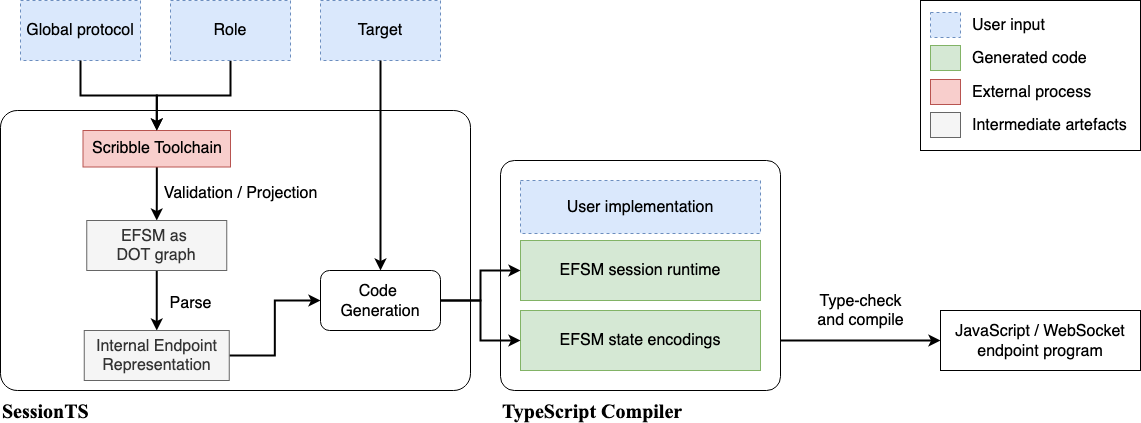
\includegraphics[width=\textwidth]{DevelopmentWorkflow}
\captionof{figure}{Overview of \fancyname{SessionTS} Development Workflow}
\label{fig:devworkflow}
\end{figure}

\subsection{Protocol Specification with Scribble}
\label{subsection:scribble}

We use the Scribble protocol description language, 
as presented in
\cite{Scribble}, for formalising the communication structure. This is
inspired by existing work on implementing session type theory 
in mainstream programming languages
\cite{Hybrid2016, PureScript2019, Python2017}. 
We use the variant of the Scribble language 
previously introduced in \cref{subsection:bgscribble}.

\subparagraph{Type declaration statements}
Specific to our TypeScript API generation toolchain,
the developer is \textit{not} required to explicitly
add type declaration statements for built-in types.
\cref{lst:adder} is a \textit{syntactically correct}
Scribble protocol as far as 
\fancyname{SessionTS} is concerned. 
Internally, \fancyname{SessionTS} inspects the protocol file
and parses existing type declarations using regular expressions
(or \textit{regex}) -- this is necessary to extract any
custom data types that will appear in the communication (for example,
\cref{lst:game}), and allows \fancyname{SessionTS} to inject
``boilerplate'' type declarations for built-in TypeScript types before
calling Scribble.

\begin{figure}[!ht]
\begin{lstlisting}[language=Scribble]
global protocol Adder(role Client, role Svr) {
	choice at Client {
		ADD(number, number) from Client to Svr;
		RES(number)         from Svr to Client;
		do Adder(Client, Svr);
	} or {
		QUIT(string) from Client to Svr;
		choice at Svr {
			THANKS()    from Svr to Client;
		} or {
			TERMINATE() from Svr to Client;
		}
	}
}
\end{lstlisting}
\captionof{lstlisting}{The \tprotocol{Adder} Protocol}
\label{lst:adder}
\end{figure}

We will use the \tprotocol{Adder} protocol as a running example
to demonstrate how our work performs TypeScript API generation.
This describes a binary session between \trole{Client} and \trole{Svr}:
if \trole{Client} asks \trole{Svr} to \tmsg{ADD} two numbers,
\trole{Svr} responds with the \tmsg{RES}ult; this loop continues
until \trole{Client} kindly asks to \tmsg{QUIT} with a message,
where \trole{Svr} either responds kindly with \tmsg{THANKS},
or just says \tmsg{TERMINATE}, but both choices will close the session.

\subsection{From Scribble to EFSM}
\label{subsection:efsm}

Given the protocol and endpoint, we use Scribble
to validate the well-formedness of the protocol and extract
information from the protocol relevant for the endpoint.
The latter is expressed as a finite state machine
where each state restricts the possible transitions, 
and transitions between states are represented by
communication actions, i.e. the sending or receiving of a message.

Scribble expresses the EFSM using the 
DOT graph description language \cite{dot}, with each
communication action encoded as the label of the corresponding
state transition. 
\fancyname{SessionTS} uses the pydot library \cite{pydot}
to parse the graph into an internal representation of the EFSM.
We define an \texttt{EfsmBuilder} class with APIs designed for
constructing the EFSM representation by iterating over the 
state transitions from the DOT representation.

\begin{figure}[!ht]
\begin{lstlisting}[language=Python]
@dataclass
class Endpoint:
    protocol: str
    role    : str
    server  : str
    efsm    : EFSM
    types   : typing.Iterable[DataType]
\end{lstlisting}
\captionof{lstlisting}{The Endpoint API}
\label{lst:endpointapi}
\end{figure}

As the code generation process requires additional information,
we define an \texttt{Endpoint} dataclass\footnote{
A Python dataclass uses the \texttt{@dataclass} decorator to generate
``boilerplate'' methods, such as the constructor, based on the
properties listed in the annotations.} (\cref{lst:endpointapi})
to contain the \texttt{EFSM}
representation, along with the information passed in from the
command line (\texttt{protocol}, \texttt{role}, \texttt{server}) 
and the custom type declarations (\texttt{types}) parsed from the
protocol specification.

\subsection{API Generation}
\label{subsection:apigen}

Formally, API generation is a function of the constructed
\texttt{Endpoint} instance
\textit{and} the target specified in the command line. We use a 
different code generation strategy for implementations running on
the server (\cref{chap:node}) versus the browser (\cref{chap:react}),
hereafter referred to as \textit{server-side endpoints} and 
\textit{browser-side endpoints} respectively.
In this subsection, we explain how we perform API generation
at a higher level of abstraction.

Traditional methods of code generation involve applying the
Visitor pattern on the internal representation. 
In the context of the MPST framework,
this may involve defining a Visitor class that implements a
\texttt{generate()} operation to be performed on the EFSM states,
such that the \texttt{generate()} implementation specialises to the
type of EFSM state, i.e. send, receive or terminal.
This is not straightforward in Python, as method overloading is not 
supported, so the ``visit'' methods would need different names.
More importantly, it is less straightforward to visualise
the structure of the generated code, as the string interpolation
aspect is likely to be interleaved with source code implementing
additional logic for code generation.

For \fancyname{SessionTS}, we leverage the Jinja \cite{jinja} 
template engine library for code generation. 
We first construct templates for the TypeScript files we wish to generate,
specifying placeholders for dynamic content (to be extracted
from the \texttt{Endpoint} object); 
we then provide Jinja with the template path and the 
\texttt{Endpoint} object, and the template engine renders the
TypeScript code by filling in the dynamic placeholders. 
We show an example in \cref{lst:jinja}.

\begin{figure}[!ht]
\begin{lstlisting}[language=javascript, title=efsm.ts.j2]
export namespace Message {

  
  export type S{{ state ~ action.label }} = {
    label: Labels.S{{ state }}.{{ action.label }},
    payload: [{{ action.payloads|join(', ') }}],
  };
  
  export type S{{ state }} = 
  | S{{ state ~ action.label }};

\end{lstlisting}
\captionof{lstlisting}{Example Jinja Template for
\fancyname{SessionTS} API Generation}
\label{lst:jinja}
\end{figure}

Jinja provides lightweight syntax for injecting content and
markup for simple control structure: \texttt{\{\{ state \}\}} 
denotes a placeholder for Jinja to render the \texttt{state} variable,
and the \texttt{\{\% \%\}} syntax  is used for conditionals and
control structures 
(such as for loops, to dynamically render the enclosing ``sub-template''
by iterating over a collection).
The main advantage that Jinja brings is that 
it decouples the ``presentation''
from the ``content'' and makes it quick to prototype and extend
the generated code, \textit{usually} without modifications to the 
code generator.

\begin{figure}[!ht]
\begin{lstlisting}[language=python]
class CodeGenerationStrategy(ABC):

    target_to_strategy = {} (*@\label{line:mapping}@*)

    def __init__(self):
        super().__init__()

    @classmethod
    def __init_subclass__(cls, *, target):
        CodeGenerationStrategy.target_to_strategy[target] = cls (*@\label{line:register}@*)
        return super().__init_subclass__()
    
    @abstractmethod
    def generate(self, endpoint: Endpoint):
        pass
\end{lstlisting}
\captionof{lstlisting}{Implementing \texttt{CodeGenerationStrategy}}
\label{lst:codegenerationstrategy}
\end{figure}

As we generate a different set of TypeScript artefacts depending
on the specified target, we structure the different code generators
using the Strategy design pattern. Each target extends the
abstract base class \texttt{CodeGenerationStrategy} 
and implements its own \texttt{generate()}
method to return a list of \texttt{(path, content)} tuples. 
We define a \texttt{CodeGenerator} class that is parameterised 
by \texttt{target}: when instantiated, it will select and perform 
the specialised \texttt{generate()} method based on \texttt{target}, 
before formatting and committing the generated code 
to the file system.
We implement a subclass hook in \texttt{CodeGenerationStrategy}
(\cref{lst:codegenerationstrategy}),
such that each derived class must provide the target name to
``register'' with the base class (\cref{line:register}),
and the base class keeps an internal
mapping of the concrete strategies (\cref{line:mapping}); 
\texttt{CodeGenerator} accesses
this mapping to select the appropriate strategy.
